\section{Results and Discussion}
\label{sec:results}
We first provide the results of the case study. Then we give more general results about the application of conflict-measuring methods to multiple multi-objective systems.

\subsection{Case Study Results}
We parameterized and solved the multi-objective model (\eqref{eqn:objFire}-\eqref{eqn:constraintNonNeg}) for each of the climate scenarios, generating three efficient frontiers: $Z_{\text{None}}$, $Z_{E45}$, and $Z_{E85}$ for the None, Ensemble RCP 4.5, and Ensemble RCP 8.5 scenarios, respectively. The frontiers are shown in Figure \ref{fig:frontiersAll}; their summary details are shown in Table \ref{tab:frontiersSummary}.

\begin{table}[]
\centering
\caption[Summary of efficient frontiers]{Summary of the performance of the efficient frontiers for each climate change scenario.}
\label{tab:frontiersSummary}
\begin{tabular}{lllll}
\multicolumn{2}{l|}{}                                                  & \textbf{None} & \textbf{E45} & \textbf{E85} \\ \hline
\multicolumn{2}{l|}{\textbf{Hypervolume}}                              & 0.876977      & 0.866857     & 0.829541     \\ \hline
\multirow{3}{*}{\textbf{Fire hazard}}       & \multicolumn{1}{l|}{min} & 21321.21      & 23219.82     & 23268.02     \\
                                            & \multicolumn{1}{l|}{max} & 21933.29      & 23973.79     & 23724.98     \\
                                            & \multicolumn{1}{l|}{avg} & 21406.26      & 23324.41     & 23369.57     \\ \hline
\multirow{3}{*}{\textbf{NSO habitat}}       & \multicolumn{1}{l|}{min} & 2532.33       & 2412.18      & 2171.10      \\
                                            & \multicolumn{1}{l|}{max} & 2540.05       & 2477.18      & 2481.01      \\
                                            & \multicolumn{1}{l|}{avg} & 2536.31       & 2447.92      & 2421.99      \\ \hline
\multirow{3}{*}{\textbf{Sediment delivery}} & \multicolumn{1}{l|}{min} & 0             & 0            & 0            \\
                                            & \multicolumn{1}{l|}{max} & 24.57         & 63.43        & 69.68        \\
                                            & \multicolumn{1}{l|}{avg} & 10.25         & 27.98        & 31.19        \\ \hline
\multicolumn{2}{l}{\textbf{Number of solutions}}                       & 51            & 701          & 1083        
\end{tabular}
\end{table}


\begin{figure}[ht!]
  \subfloat[None]{%
    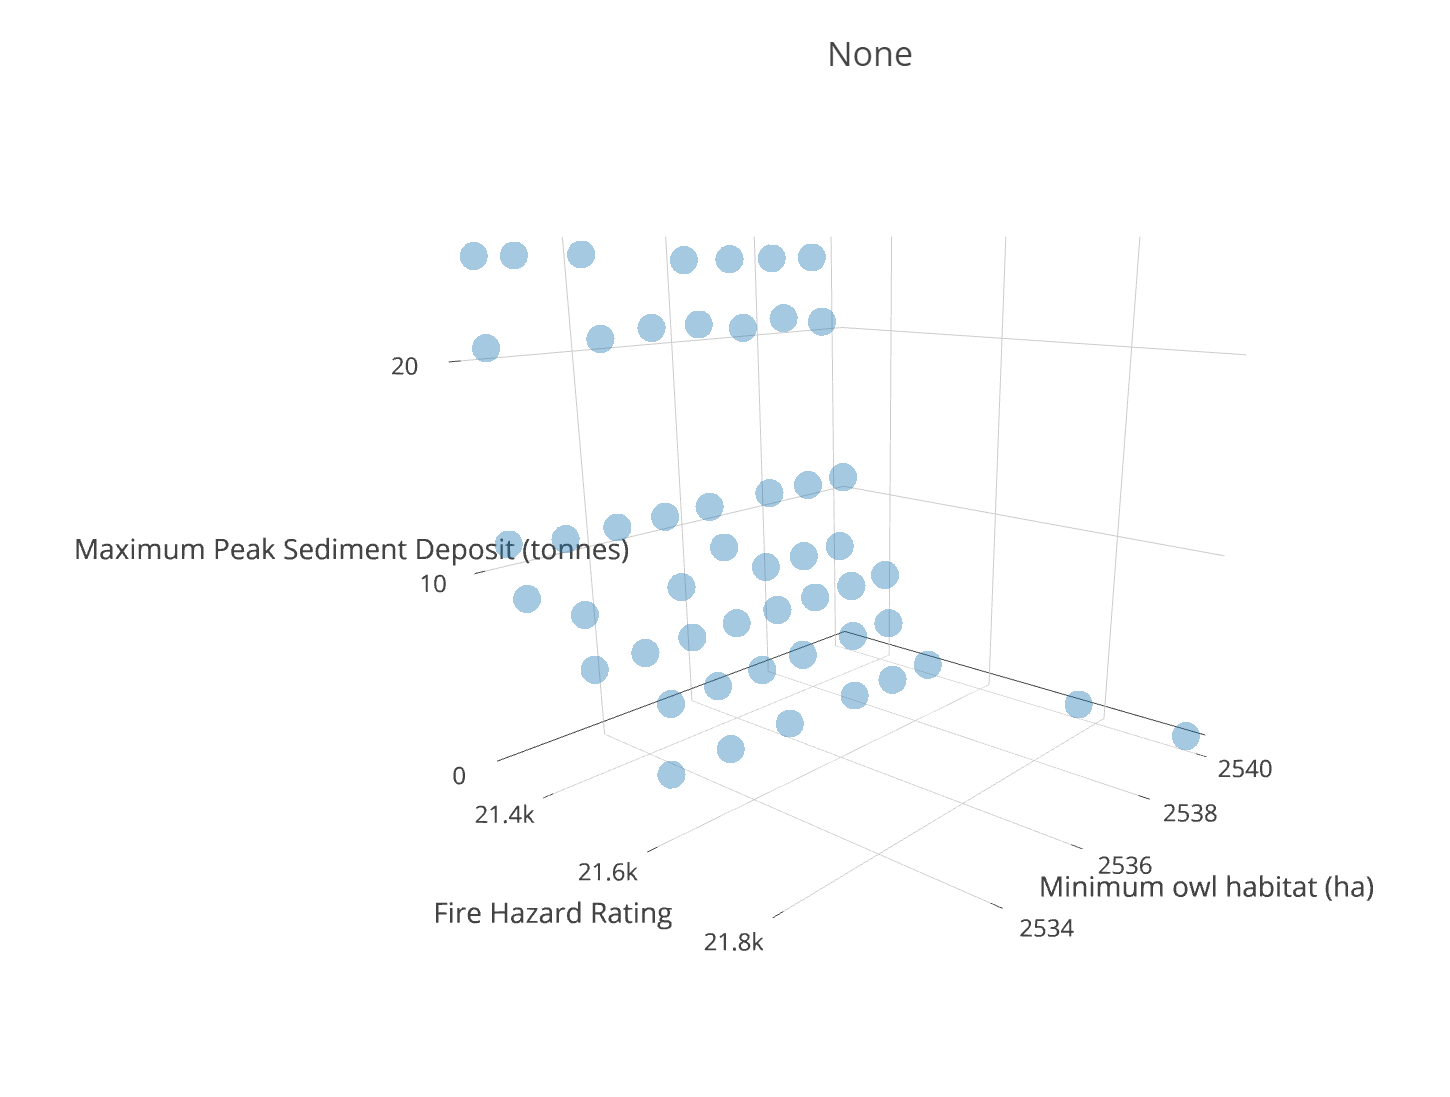
\includegraphics[width=.45\textwidth]{../images/Frontier_None}%
    \label{fig:frontierNone}%
  }
  \subfloat[Ensemble RCP 4.5]{%
    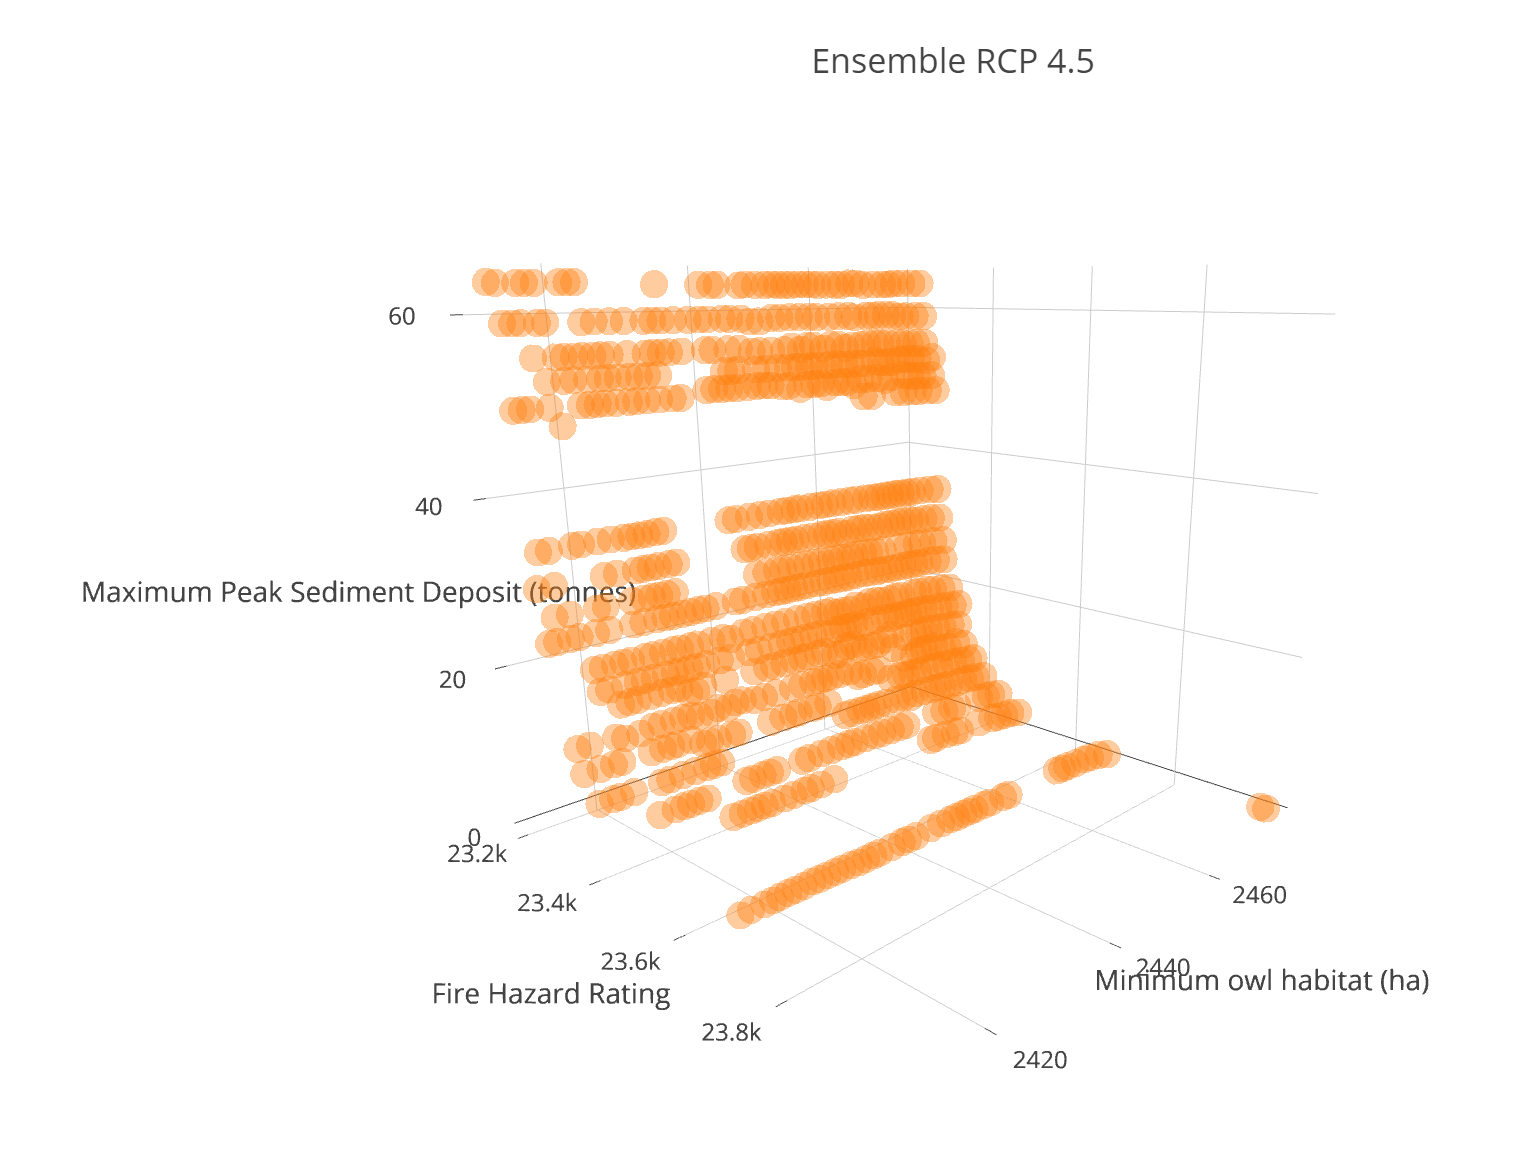
\includegraphics[width=.45\textwidth]{../images/Frontier_E45}%
    \label{fig:frontierE45}%
  }\hfill\centering
  \subfloat[Ensemble RCP 8.5]{%
    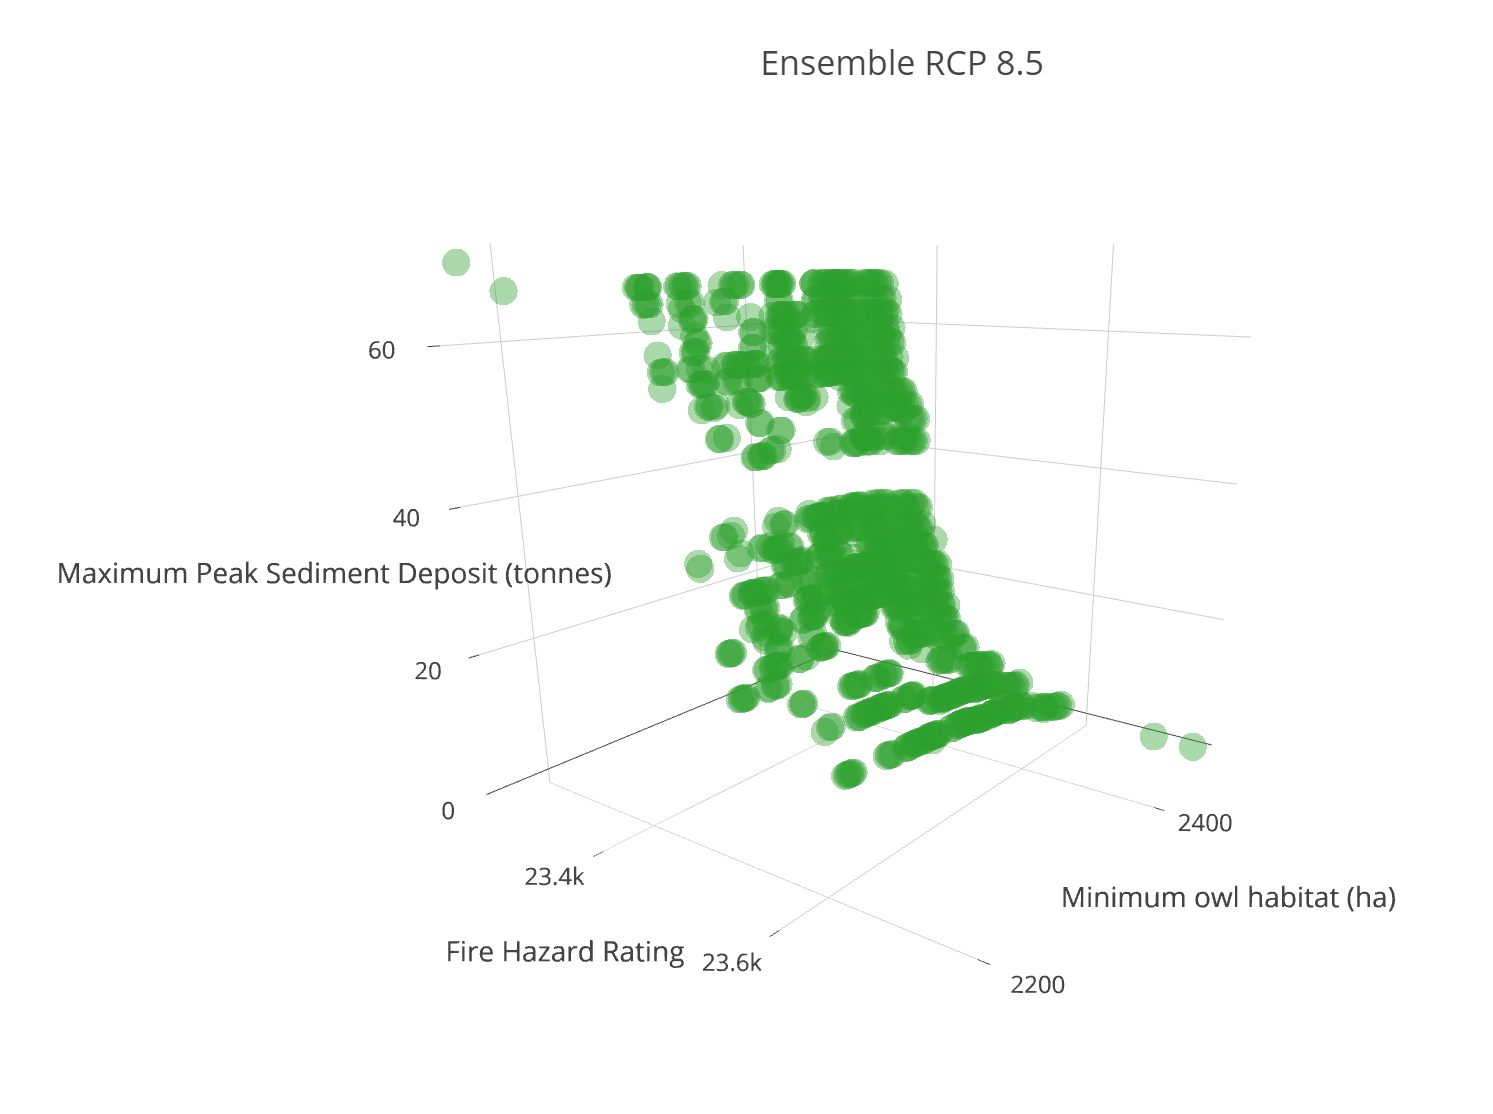
\includegraphics[width=.45\textwidth]{../images/Frontier_E85}%
    \label{fig:frontierE85}%
  }
  \caption[Frontiers for each climate change scenario]{Efficient frontiers for each climate change scenario.}
  \label{fig:frontiersAll}
\end{figure}

We begin our analysis by investigating the impacts of climate change on the provision of individual ecosystem services. We then consider how climate change impacts the joint provision of ecosystem services and the conflict among them.

\subsubsection{Individual ecosystem service achievement}
The average achievement of all ecosystem services decreases with increasing severity of climate change (see Table \ref{tab:frontiersSummary}, ``avg'' rows). We find the difference in ecosystem service provision greater between the assumption of no climate change and mild climate change (None to E45) than it is between mild climate change and severe climate change (E45 to E85). This suggests that, for the ecosystem services in this study, the realization of climate change is more significant than the severity of that change.

The model data provide evidence of why this is the case. Consider Figure \ref{fig:avgSedimentDelivery}. This figure shows the average number of tonnes of sediment delivered as a result of performing fuel removals for each climate change scenario. The sediment delivery under E45 is nearly twice the sediment delivery under the None scenario (81\% higher), whereas the E85 scenario is only 0.4\% higher than the E45 scenario.

We trace this phenomenon back to the sediment delivery response to prescribed burns and the frequency with which they are assigned. While the sediment delivery response to thinnings is similar across climate scenarios, the response to prescribed burns is more pronounced. We also find that relative to the None scenario, prescribed burns are assigned 8 times more frequently in E45 and 10.1 times more frequently in E85. See Table \ref{tab:prscBurnsInClimChange}. These effects combine to produce the result seen in Figure \ref{fig:avgSedimentDelivery}. For additional information on how stands are assigned a specific fuel removal techniques such as thinning or prescribed burn, see the appendix, \S \ref{chap:appendix_drinkTreatments}.

\begin{figure}[ht]
\centering
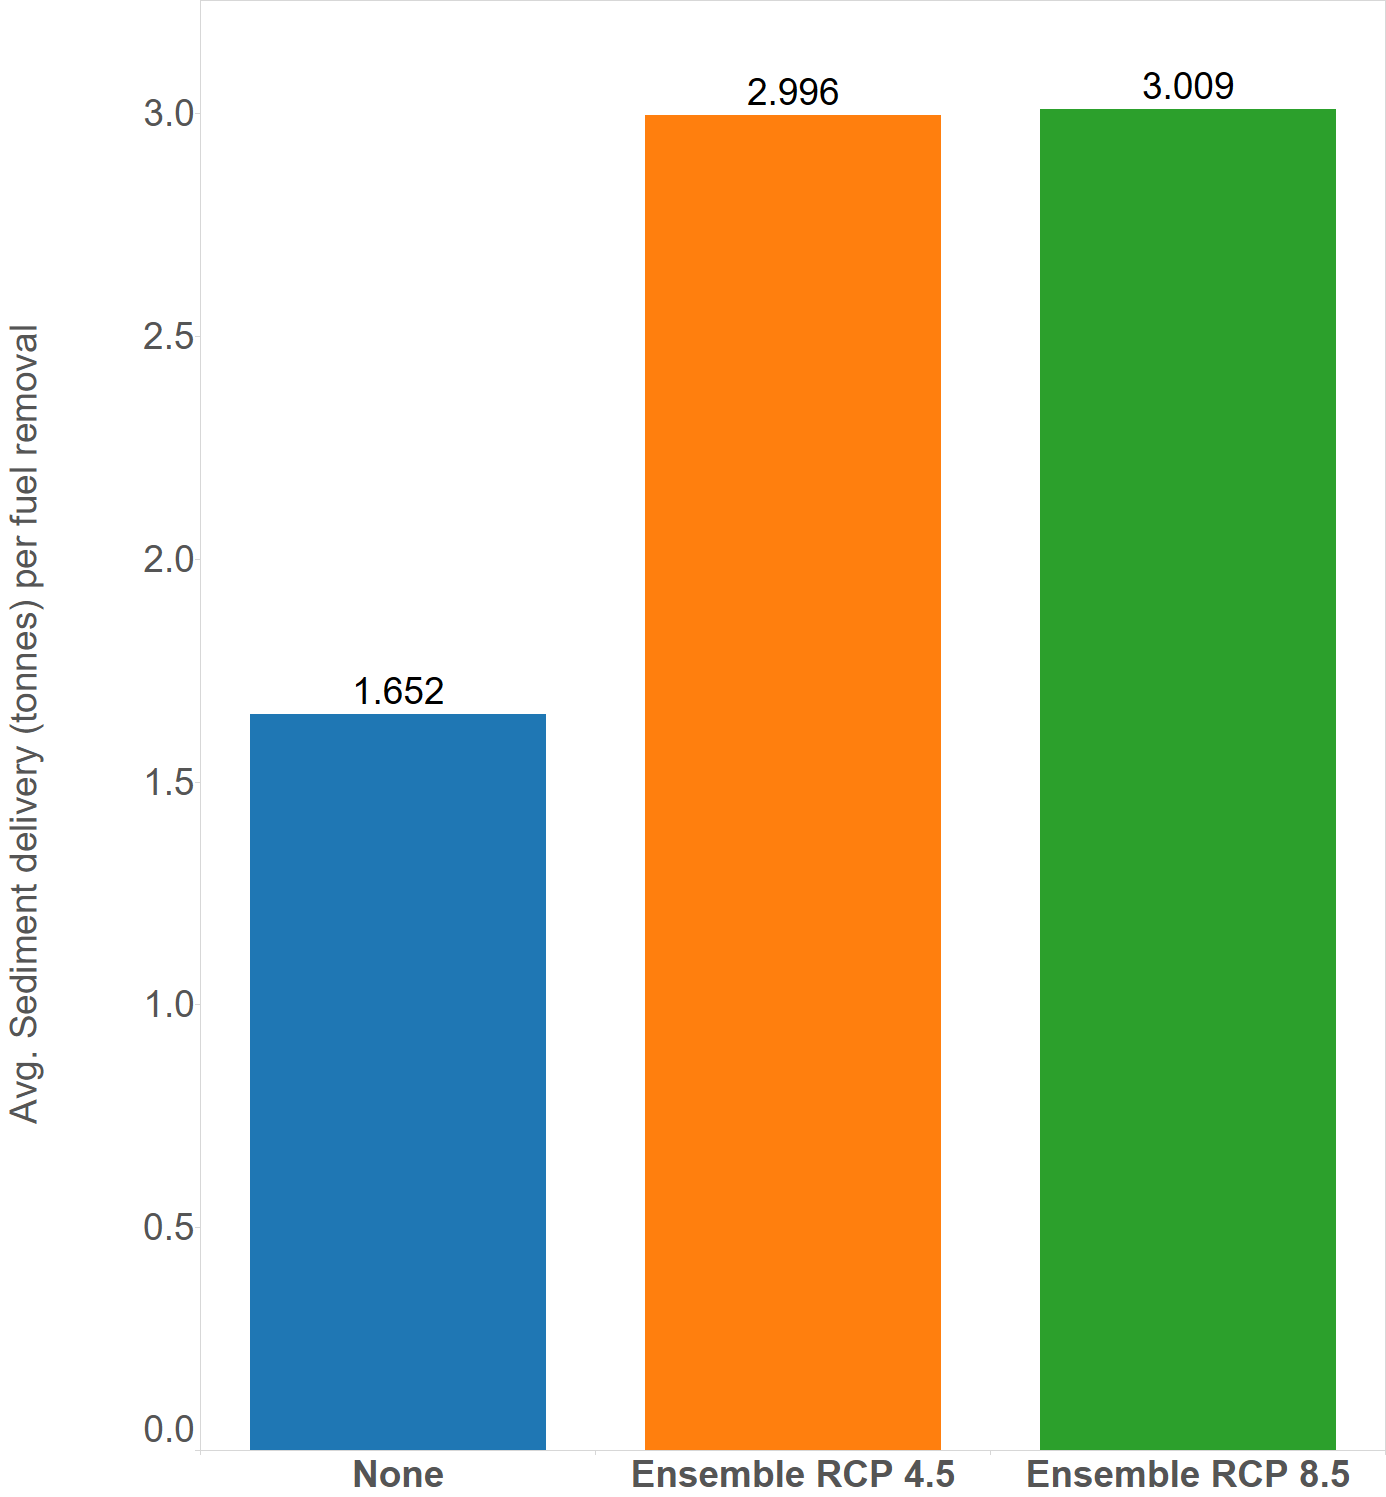
\includegraphics[width=.55\textwidth]{../images/AvgSedimentSpikes}
\caption[Average sediment delivery across climate scenarios]{Average spike in sediment delivery as a result of performing fuel removals for each of the climate change scenarios.}
\label{fig:avgSedimentDelivery}
\end{figure}

\begin{table}[]
\centering
\caption[Frequency and impact of prescribed burns for each climate scenario]{Frequency and impact of prescribed burn for each climate scenario. The combination of more frequent prescribed burns and increased sediment delivery per prescribed burn results in the higher values of sediment delivery in E45 and E85 observed in Figure \ref{fig:avgSedimentDelivery}.}
\label{tab:prscBurnsInClimChange}
\begin{tabular}{l|lll}
                                                                                                           & \textbf{None} & \textbf{E45} & \textbf{E85} \\ \hline
\textbf{\begin{tabular}[c]{@{}l@{}}Average sediment delivery\\ (tonnes) from prescribed burn\end{tabular}} & 31.23            & 48.56          & 48.97          \\
\textbf{\begin{tabular}[c]{@{}l@{}}Number of prescribed\\ burns assigned\end{tabular}}                     & 34         & 272        & 344       
\end{tabular}
\end{table}

Similarly, consider Figure \ref{fig:cumSmallestFireHazard}. For each climate scenario, the figure shows the resulting fire hazard of the Drink Area if the most successful fire hazard reduction techniques were performed. We again notice increased fire hazard of the Drink Area as a result of climate change, with a larger difference between None and E45 than between E45 and E85. This is due to more stands in the Drink Area having a fuel model classification that is associated with higher fire hazard under climate change scenarios E45 and E85 than in the case of None. This trend is shown in Figure \ref{fig:distOfFireHazards}, where we observe a larger percentage of stands having a fire hazard rating of either 4 or 5 under the E45 and E85 scenarios than in None.

\begin{figure}[ht]
\centering
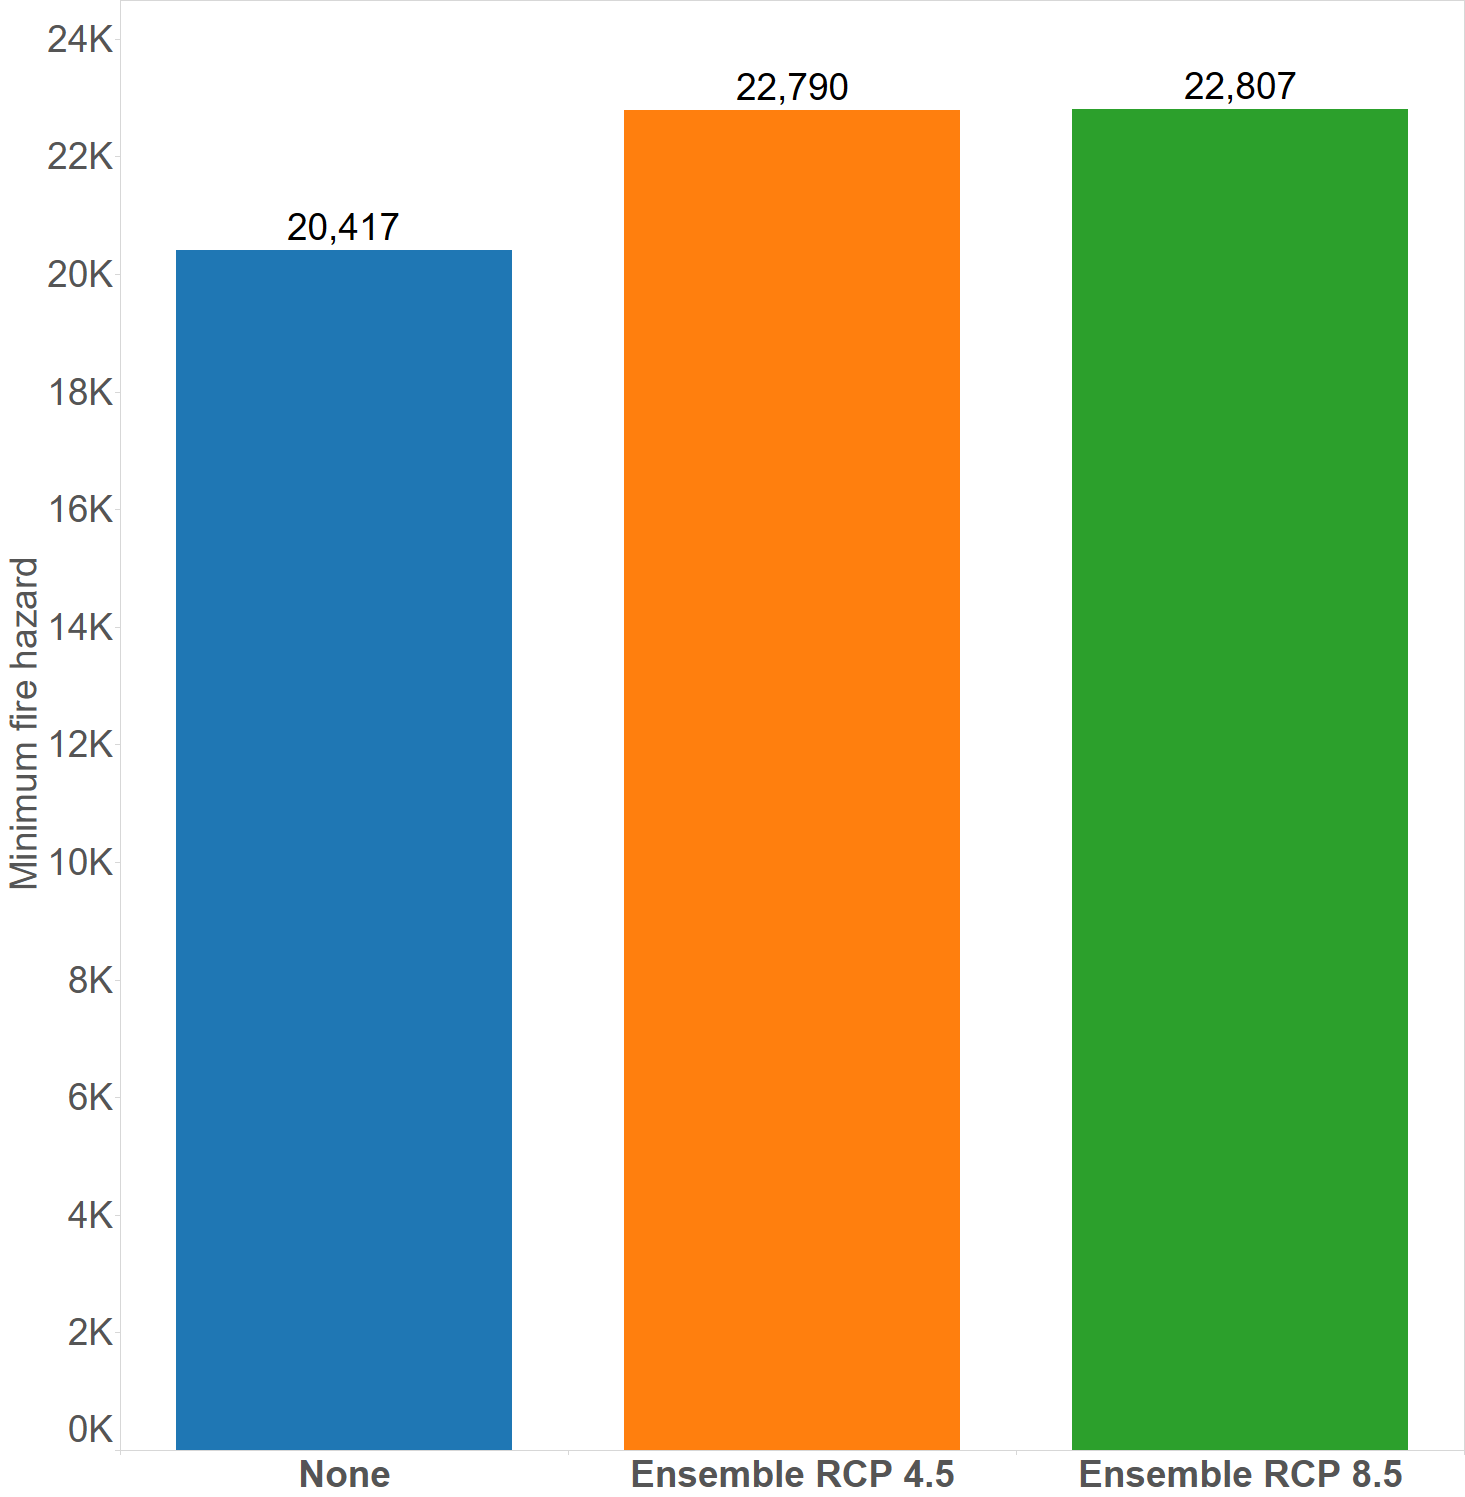
\includegraphics[width=.40\textwidth]{../images/CumSmallestFireHazard}
\caption[Lower bound on fire hazard for each climate scenario]{Shown here are lower bounds on the minimum fire hazard for the Drink Area under each climate change scenario. They represent the cumulative fire hazard of the Drink Area if the most extreme fire hazard reduction techniques were employed without regard to the constraints on fuel removals (inequalities \eqref{eqn:constraintAreaRestr}-\eqref{eqn:constraintAreaFlucU}).}
\label{fig:distOfFireHazards}
\end{figure}

\begin{figure}[ht]
\centering
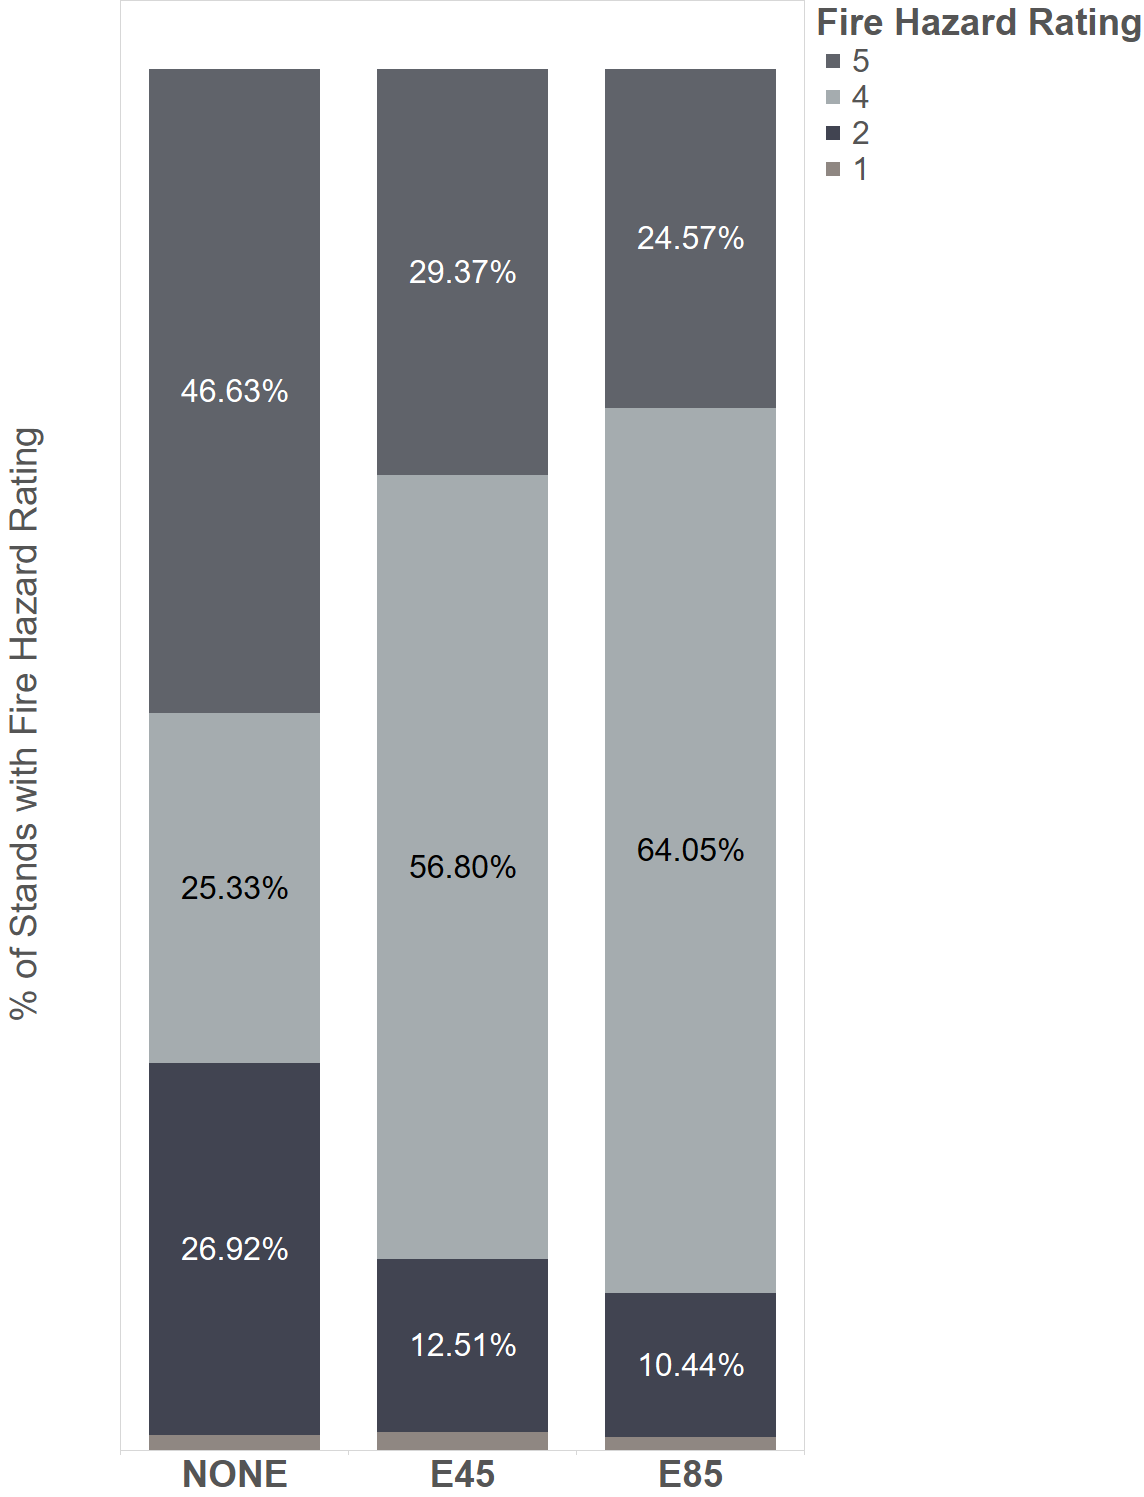
\includegraphics[width=.5\textwidth]{../images/FireHazardRatingsPerClimateScenario}
\caption[Distribution of fire hazard ratings over the Drink Area for each climate change scenario]{Distributions of fire hazard ratings across the Drink Area under each climate change scenario. Moving from left to right (in increasing climate change severity), we observe an increase in the number of stands classified with more extreme fire hazards (ratings of 4 and 5).}
\label{fig:cumSmallestFireHazard}
\end{figure}

The same holds true for NSO habitat. From the values in Table \ref{tab:nsoHabDQs} that fuel removals more frequently disqualify a stand from being NSO habitat under the climate change scenarios than for None.

\begin{table}[ht]
\centering
\caption[Frequency of NSO habitat disqualifications for each climate scenario]{Shown here are the number of times for each climate scenario that a fuel removal triggers the disqualification of a stand from being NSO habitat.}
\label{fig:nsoHabDQs}
\begin{tabular}{l|l}
\textbf{Climate change scenario} & \begin{tabular}{@{}l@{}}\textbf{Disqualifications of NSO habitat} \\ \textbf{as a result of fuel removals}\end{tabular} \\ \hline
\textbf{None}                    & 24                                                                               \\
\textbf{Ensemble RCP 4.5}        & 60                                                                               \\
\textbf{Ensemble RCP 8.5}        & 60                                                                              
\end{tabular}
\end{table}

% Talk about sources of conflict in between objectives. Well, the conflict metric is higher for this frontier than for this frontier (graph of cross section). The underlying reason for this is bc the ?sed contrib is higher in this scenario than that scenario? or ?the efficacy of treatments is highest in E85 and on the stands located in the watershed?. Something like that. Look into treatment efficacy on WS stands across the climate scenarios. And the sediment contributions vs climate scenarios.

% Per stand, avg reduction in fire hazard vs sediment delivered as a result of fuel removal (same thing for reduc in fire hazard vs triggering NSO habitat)

% For a given fuel removal that disqualifies a stand as NSO habitat, what is the difference in fire hazard between the "NONE" and (whatever that fuel removal action was) is?